\section{Gundlagen}

MPPT Solar





\section{Entwurf}

In diesem Kapitel wird der Entwurfsprozess und die Planung des Systems thematisiert.
Zuerst wurden Anforderungen und Rahmenbedingungen festgelegt, unter denen das System Anwendung findet. Um die Funktionsblöcke zu definieren, wurden Blockschaltbilder und Zustandsdiagramme genutzt. Das Design wurde mit einem Prototyp getestet, und später als \ac{PCB} fertiggestellt.

Ziel Festlegen
Grobes Blockschaltbild
Recherchieren nach Teilen (für die Blöcke) (Datenblätter etc)
Prototyp Bauen, und Analysieren, Testen (Solar schonmal etc)
PCB - Designen, fertigen lassen
PCB testen und Verbessern
?Iteration V2 vom PCB?
Generelle Tests
Auswertung

\subsection{Anforderungen}
\begin{itemize}
    \item Autonom Betrieben / Solar - Batterie
    \item Eigenständig / Keine Wartung (keine Batterie austauschen / Daten persönlich einsammeln etc)
    \item Schnittstellen für Sensoren und Aktuatoren via \ac{GPIO} / \ac{ADC} 
    \item Datenweiterleitung an Server / Internet via Relays oder Direkt
    \item DIY - Kosteneffizient, nicht zu teure Teile
    \item Operation auch in abgelegenen Orten
    \item Periodische Messung, keine Echtzeitanwendung
    \item Mit so wenig Strom wie möglich, Power Effizient
\end{itemize}

\subsection{Modulliste / Komponentenfestlegung}
Die Anforderungen wurden in eine Liste an Komponenten übersetzt, welche die Funktionalitäten erfüllen.

\subsubsection{Stromversorgung}
Die Stromversorgung ist essentiell für die Operation des Systems.

Akku

\begin{table}[h!]
    \centering
    \begin{tabular}{cccc}
         &  Angegeben&  Gemessen& \\
         Kapazität&  10Ah / 37Wh&  8.6Ah / 30Wh& \\
         Spannung&  3.2-4.2V&  3.2-4.2V& \\
         Innenwiderstand?&  &  & \\ 
 Größe& & &\\
 Gewicht& & &\\
    \end{tabular}
    \caption{Akkuwerte}
    \label{tab:placeholder}
\end{table}

Für eine hohe Energiedichte, Maximalstrom und möglichst geringes Gewicht wurde auf einen \ac{LiPo}-Akku gesetzt.
Ein 10Ah Akku mit 37Wh wurde gewählt, um eine möglichst lange Operation zu gewährleisten.
Der Akku verfügt über einen integrierten Schutzchip, mit Über/Unterspannungsabschaltung und Maximalstromabschaltung.
lipo Bilder
Die \ac{Akkus} wurden auf ihre Kapazität mittels einem Kapazitätsmessgerät von Atorch getestet.
\begin{figure}
    \centering
    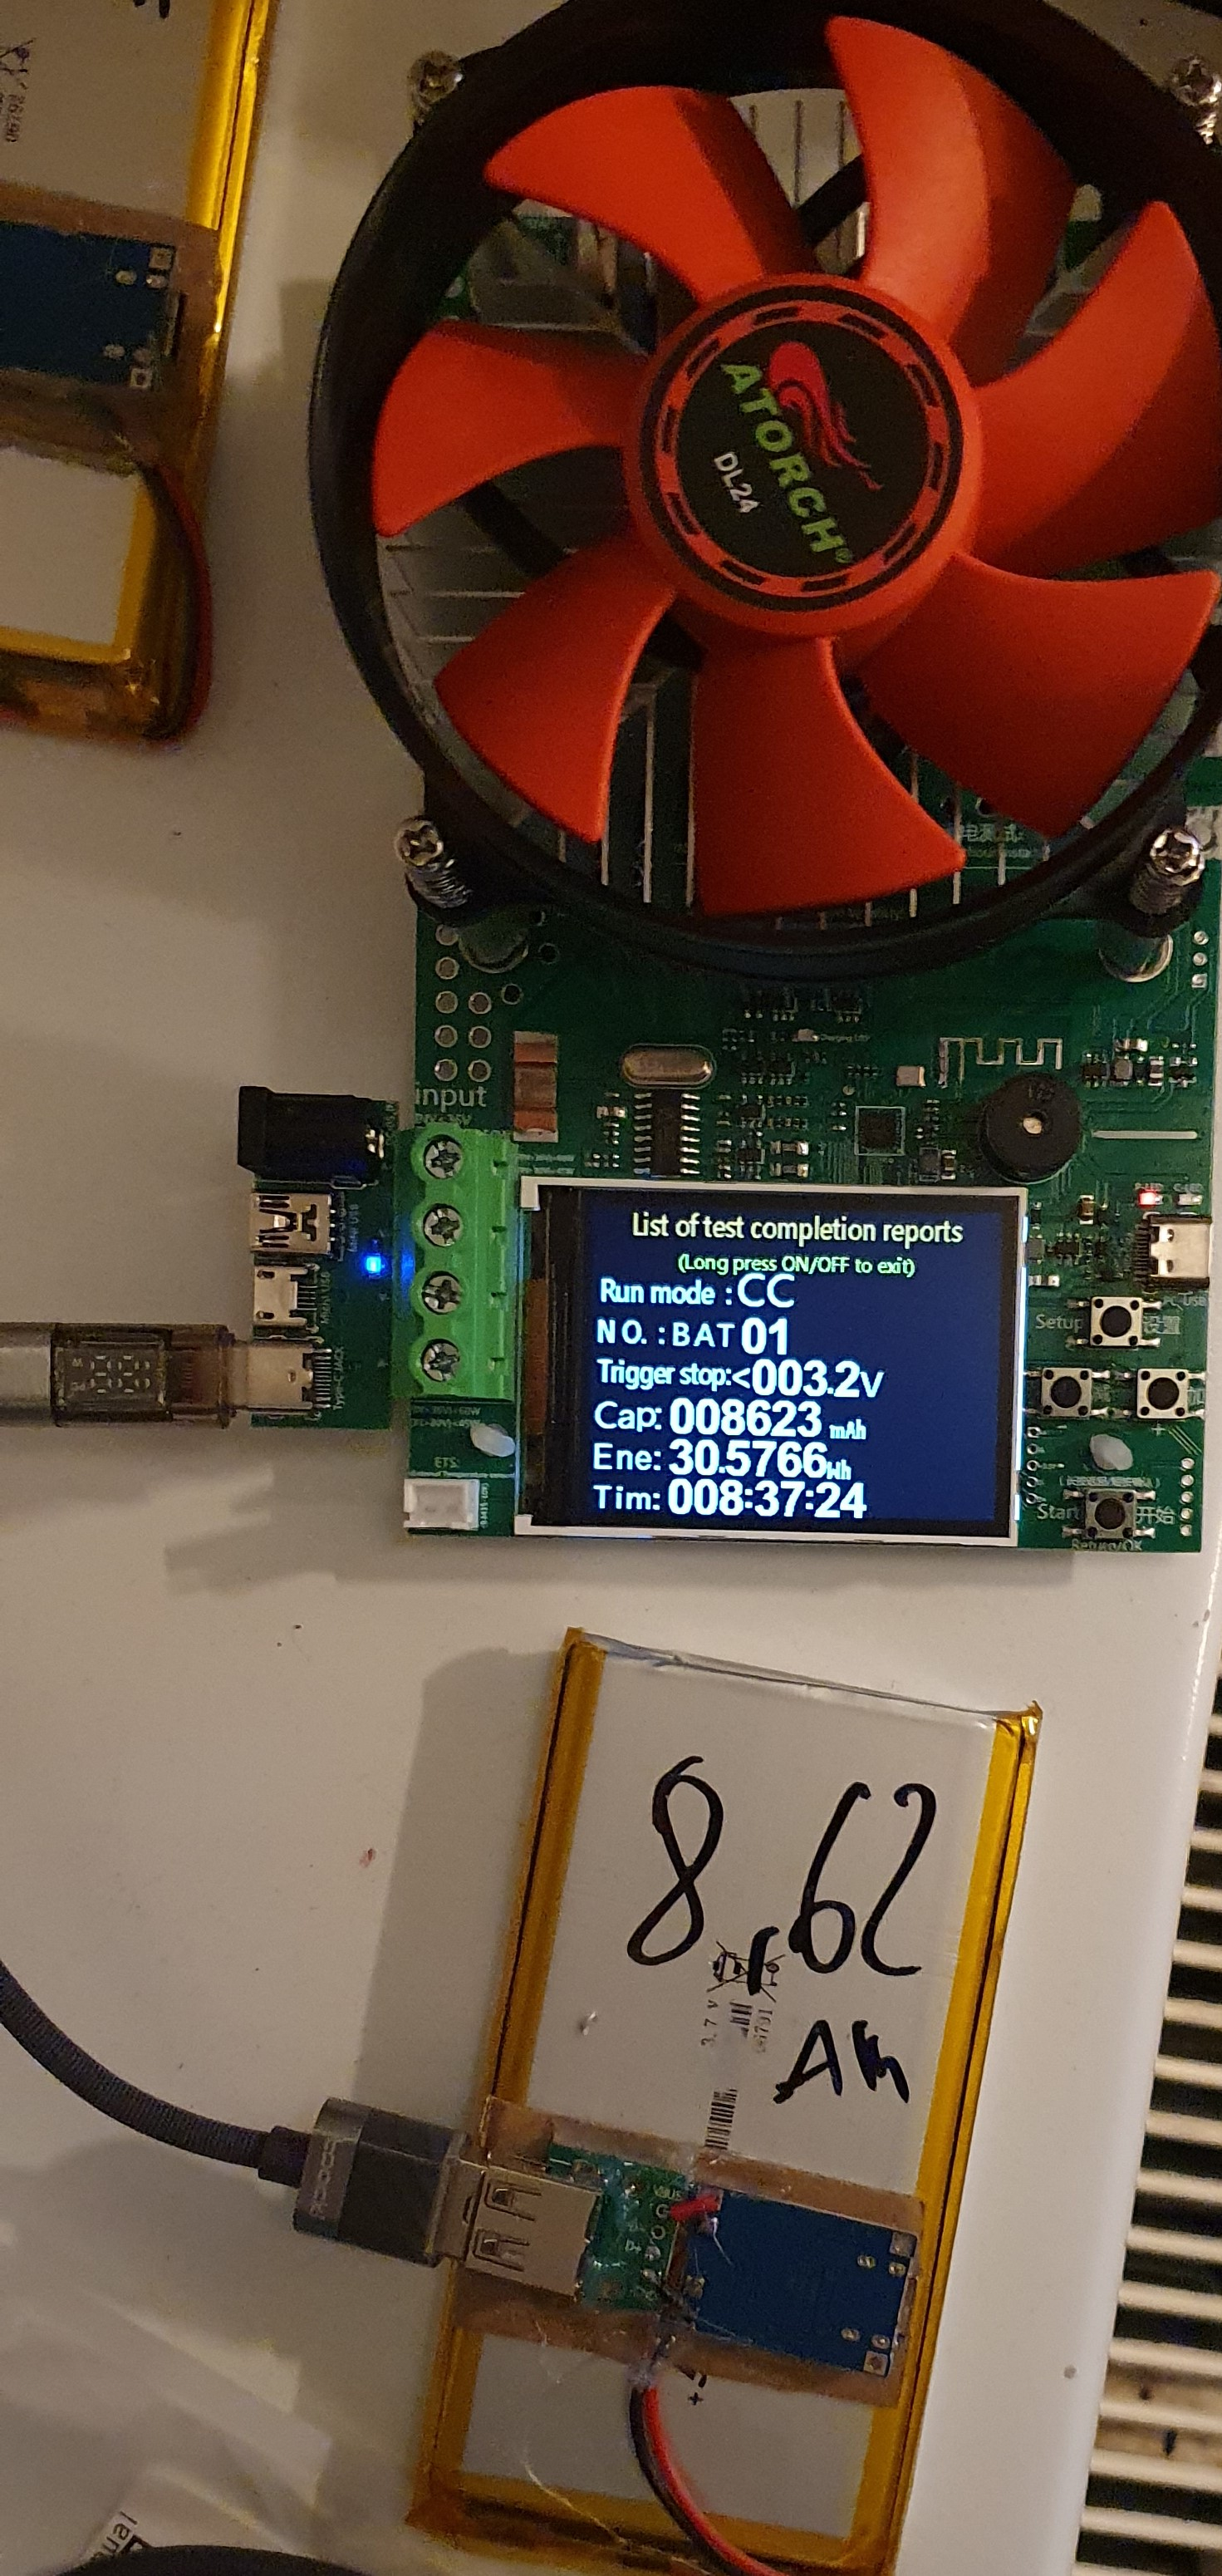
\includegraphics[width=0.5\linewidth]{img/solar_test/cap_bat.jpg}
    \caption{Batterie Kapazitätstest}
    \label{fig:cap_test}
\end{figure}

Um den Akku zu Laden wird ein Solar-Charge-Controller mit MPPT von Waveshare verwendet.
Der Ruhestrom liegt hier bei 20mA, womit der Akku nach 20 Tagen ohne Sonne leer wäre.
Wurde gewählt, wegen kompakten formfaktor, und großen Eingangsspannungsbereich.
Andere Solar-Charge-Controller mit geringerem Ruhestrom wären eine Verbesserung.

\begin{table}
    \centering
    \begin{tabular}{cccc}
         &  Waveshare Solar Charger&  Mini Solar Charger& Buck converter + 
Lipo Charger\\
         Eingangspannung V&  5-26&  6& \\
         Ruhestrom mA&  2&  & \\
         Maximalladestrom A&  &  1& \\
 Lipo Charger Integriert& Ja& Ja&Ja\\
 MPPT Tracker& Ja& Ja&Nein\\
 Effizienz \%& & &\\
 Nutzungsaufwand& Gering& Mittel&Hoch\\
    \end{tabular}
    \caption{Solar-Lademodul Vergleich}
    \label{tab:placeholder}
\end{table}


Solartests
Eine Solarzelle wurde unter Berliner Sommerbedingungen auf ihre tägliche Energieproduktion getestet. Die Tests wurden mit dem Kapazitätsmessgerät \ref{fig:atorch_load} durchgeführt.
Die variable Last wurde unter der \ac{CV} Einstellung betrieben, da diese über keinen MPPT-Controller verfügt.
Die suboptimale Nutzung des Solarstroms stellt daher eine untere Grenze für die Energiebereitstellung des Gesamtmoduls dar. Da das Waveshare-Modul mit MPPT-Controller den Gesamtstrom regeln kann, um die größtmögliche Energie zu gewinnen.


\begin{table}[h!]
    \centering
    \begin{tabular}{lc}
            Lichtverhältnisse&Wh / 1 Zelle \\
 Regen& 0-1\\
            Bewölkt&1-2\\
            Sonnig&2-5\\
    \end{tabular}
    \caption{Solartest}
    \label{tab:sol_cond}
\end{table}
Die Ergebnisse der Solarmessung bei versch. Wetterbedingungen können grob approximativ wie in \ref{tab:sol_cond} dargestellt werden. Die genauen Messreihen sind im folgenden dargestellt.

\begin{table}[h!]
    \centering
    \begin{tabular}{cccll}
         Zeit in h&  Energie in Wh& $\Delta$ T&$\Delta$ Wh &Wetter\\
         6:30&  2.77&  6:30h&2.77 &Sonnig\\
         13:00&  2.94&  6:30h&0.17 &-\\
 42:40& 3.5& 29:40& 0.56&Regen\\
 62:00& 4.1& 19:20& 0.6&-\\
 87:40& 5& 25:40& 0.9&-\\
 106:20& 6.2& 18:40& 1.2&-\\
 144:14& 6.66& 37:54& 0.46&-\\
 169:00& 7.1& 24:46& 0.44&-\\
    \end{tabular}
    \caption{Solar Messreihe 1 }
    \label{tab:sol_mess1}
\end{table}
\begin{table}[h!]
    \centering
    \begin{tabular}{cccll}
         Zeit in h&  Energie in Wh& $\Delta$ T&$\Delta$ Wh &Wetter\\
         8:30&  2.68& 8:30&2.68 &Sonnig\\
         17:00&  2.7& 8:30&0.02 &-\\
         34:00&  5.12&  17:00&2.42 &-\\
         71:20&  9.51&  37:20&4.39 &-\\
         81:25&  10.09&  10:05& 0.58&-\\
 91:25& 12:15& 10:00& 2.06&Wolkig\\
 137:40& 15.95& 46:15& 3.8&-\\
 148:51& 16.85& 11:11& 0.9&-\\
 184:20& 21.36& 35:29& 4.51&-\\
 199:40& 23.67& 15:20& 2.31&-\\
    \end{tabular}
    \caption{Solar Messreihe 2}
    \label{tab:sol_mess2}
\end{table}
\begin{table}[h!]
    \centering
    \begin{tabular}{cccll}
         Zeit in h&  Energie in Wh&  $\Delta$ T& $\Delta$ Wh &Wetter\\
         9:55&  0.5&  9:55& 0.5&Wolkig\\
         50:39&  3.65&  40:44& 3.15&Sonnig\\
 80:15& 6.64& 29:36& 2.99&-\\
 84:36& 6.70& 4:21& 0.06&-\\
 93:13& 8.49& 8:37& 1.79&-\\
 148:31& 18.84& 55:18& 10.35&-\\
 159:51& 22.22& 11:20& 3.38&-\\
    \end{tabular}
    \caption{Solar Messreihe 3}
    \label{tab:sol_mess3}
\end{table}

\begin{figure}[h!]
    \centering
    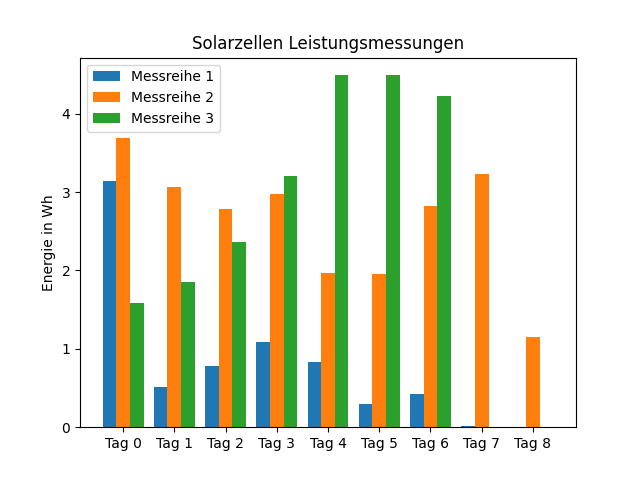
\includegraphics[width=0.8\linewidth]{img/solar_test/Solar_leistung.png}
    \caption{Solar Leistungsmessung - Durchschnitt pro Tag}
    \label{fig:solar_power}
\end{figure}
\footnote{Da die Zeitpunkt der Messung, sowie der Messstartpunkt stark variierten ist hier keine präzise Bestimmung der Leistung zu einem speziellen Tag angestrebt. Durchaus aber ein Durchschnitt pro Tag.}


Low Power
Das System soll um Energieeffizient zu arbeiten, alle nicht benötigten Module ausschalten.
Der Adafruit Timer schaltet das gesamte System in einem Intervall von 2 Stunden an, und der \ac{MCU} signalisiert dem Timer Board über den Done Pin, wann der Mess- und Uploadvorgang beendet, und das System wieder auszuschalten ist.


Strommessungen des Systems

Um den Stromverbrauch des Gesamtsystems zu bestimmen wurde ein USB-Strommessgerät von FNIRSI genutzt.

\begin{figure}[h!]
    \centering
    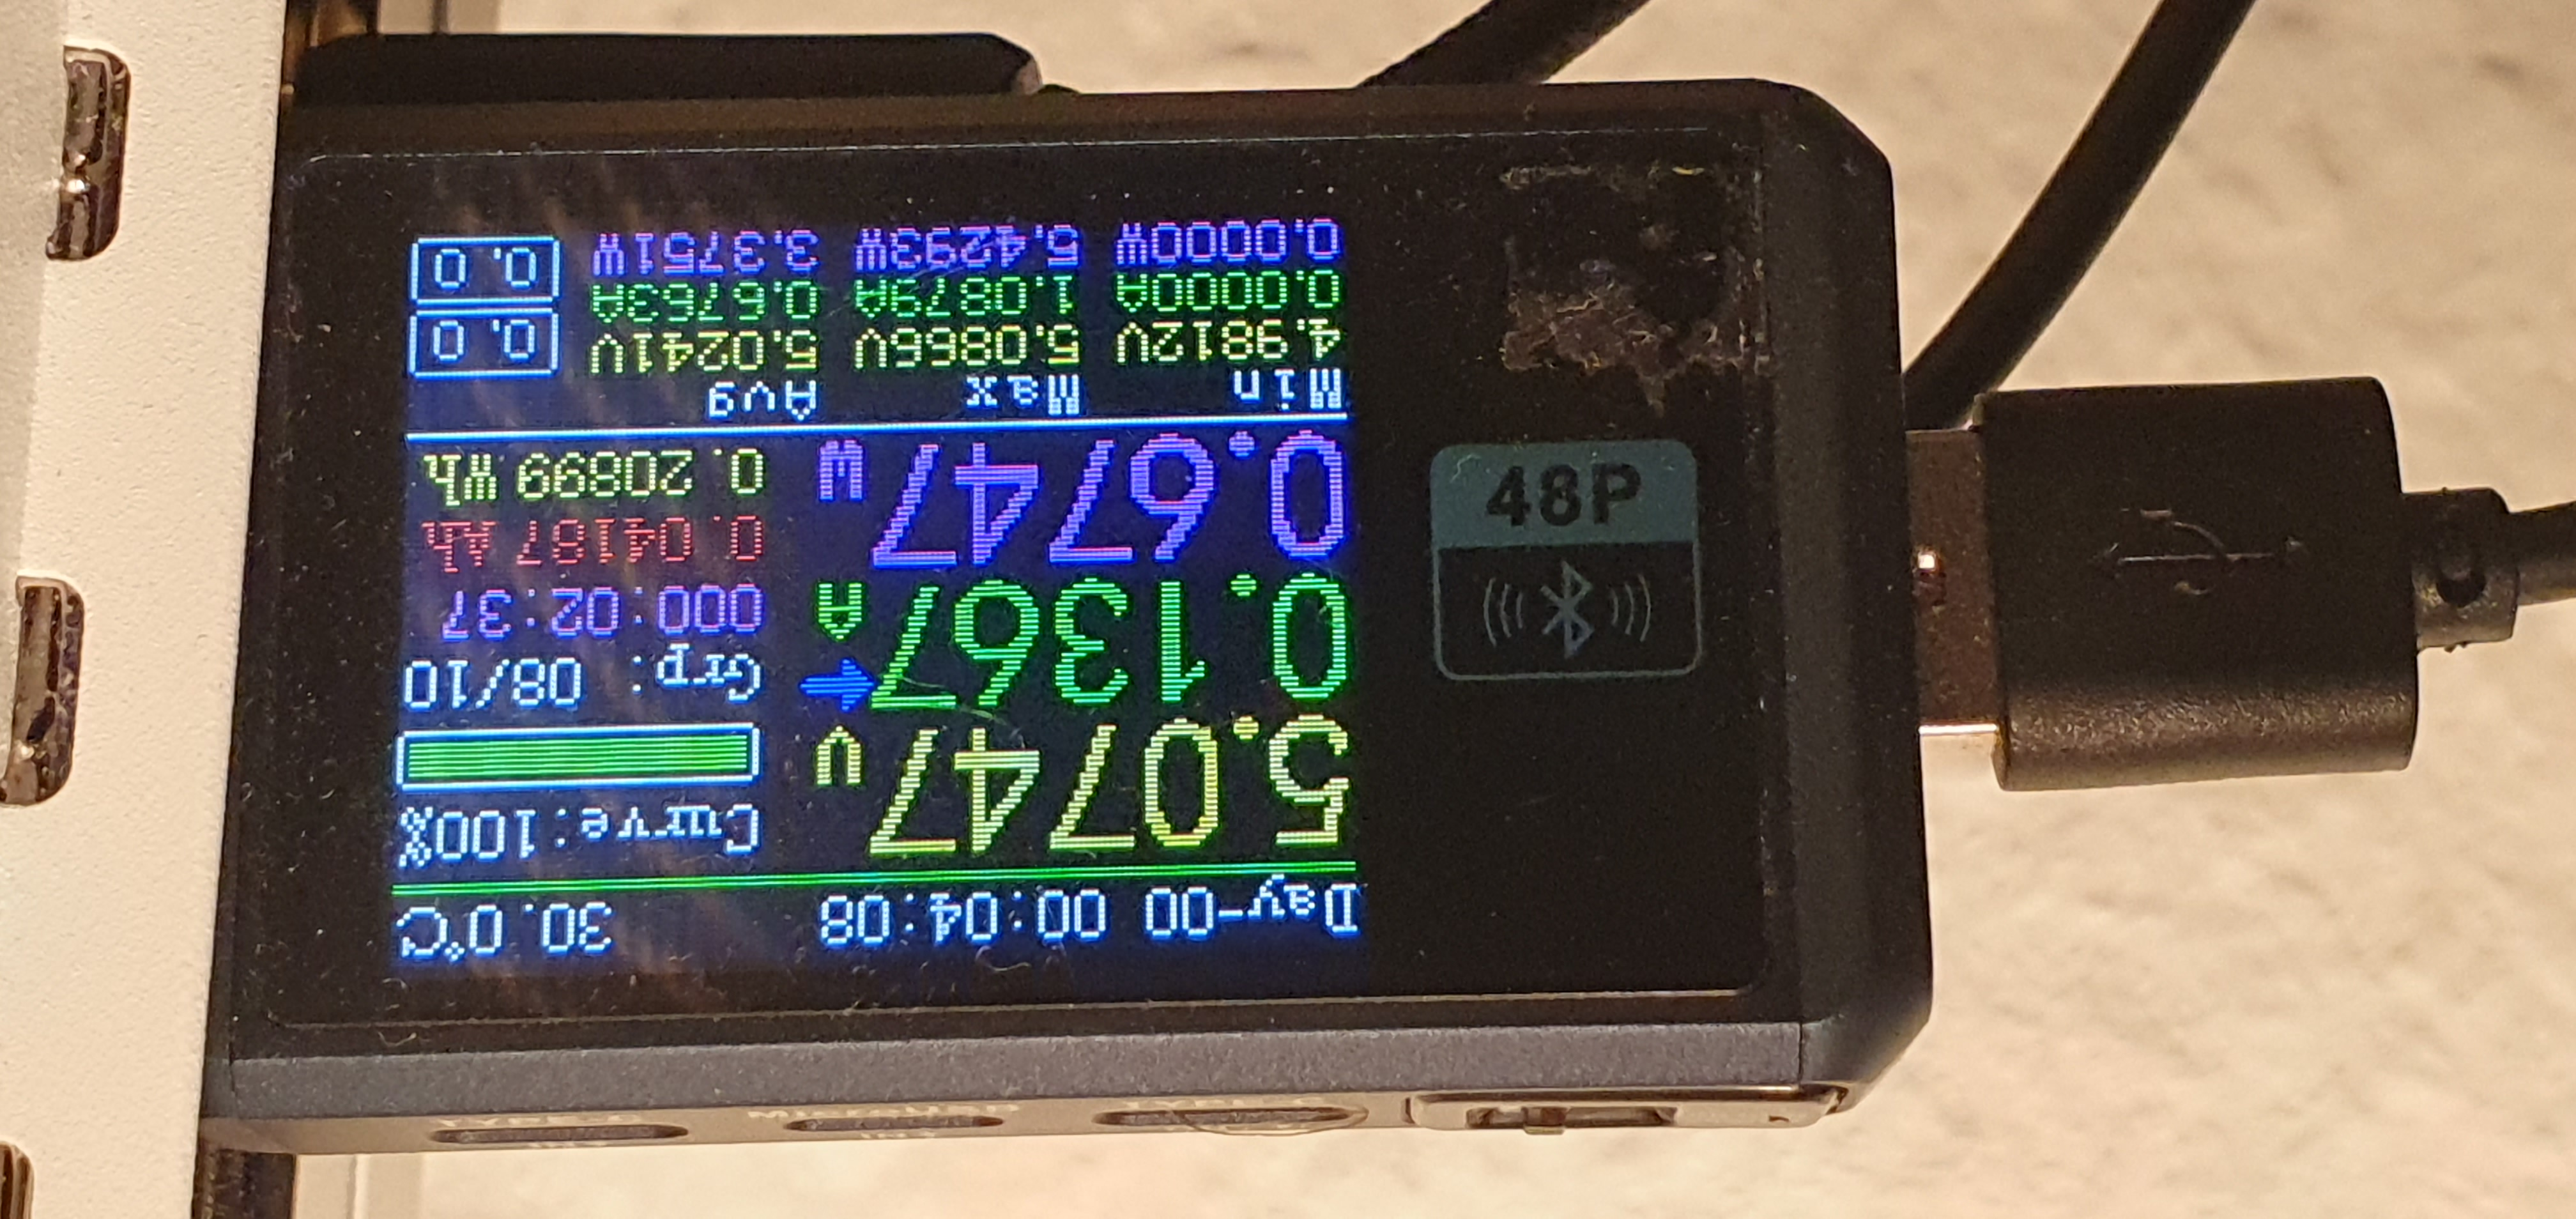
\includegraphics[width=0.5\linewidth, angle=180]{img/power_test/idle.jpg}
    \caption{Leistungsaufnahme im Messzustand}
    \label{fig:pwr_idle}
\end{figure}
\begin{figure}[h!]
    \centering
    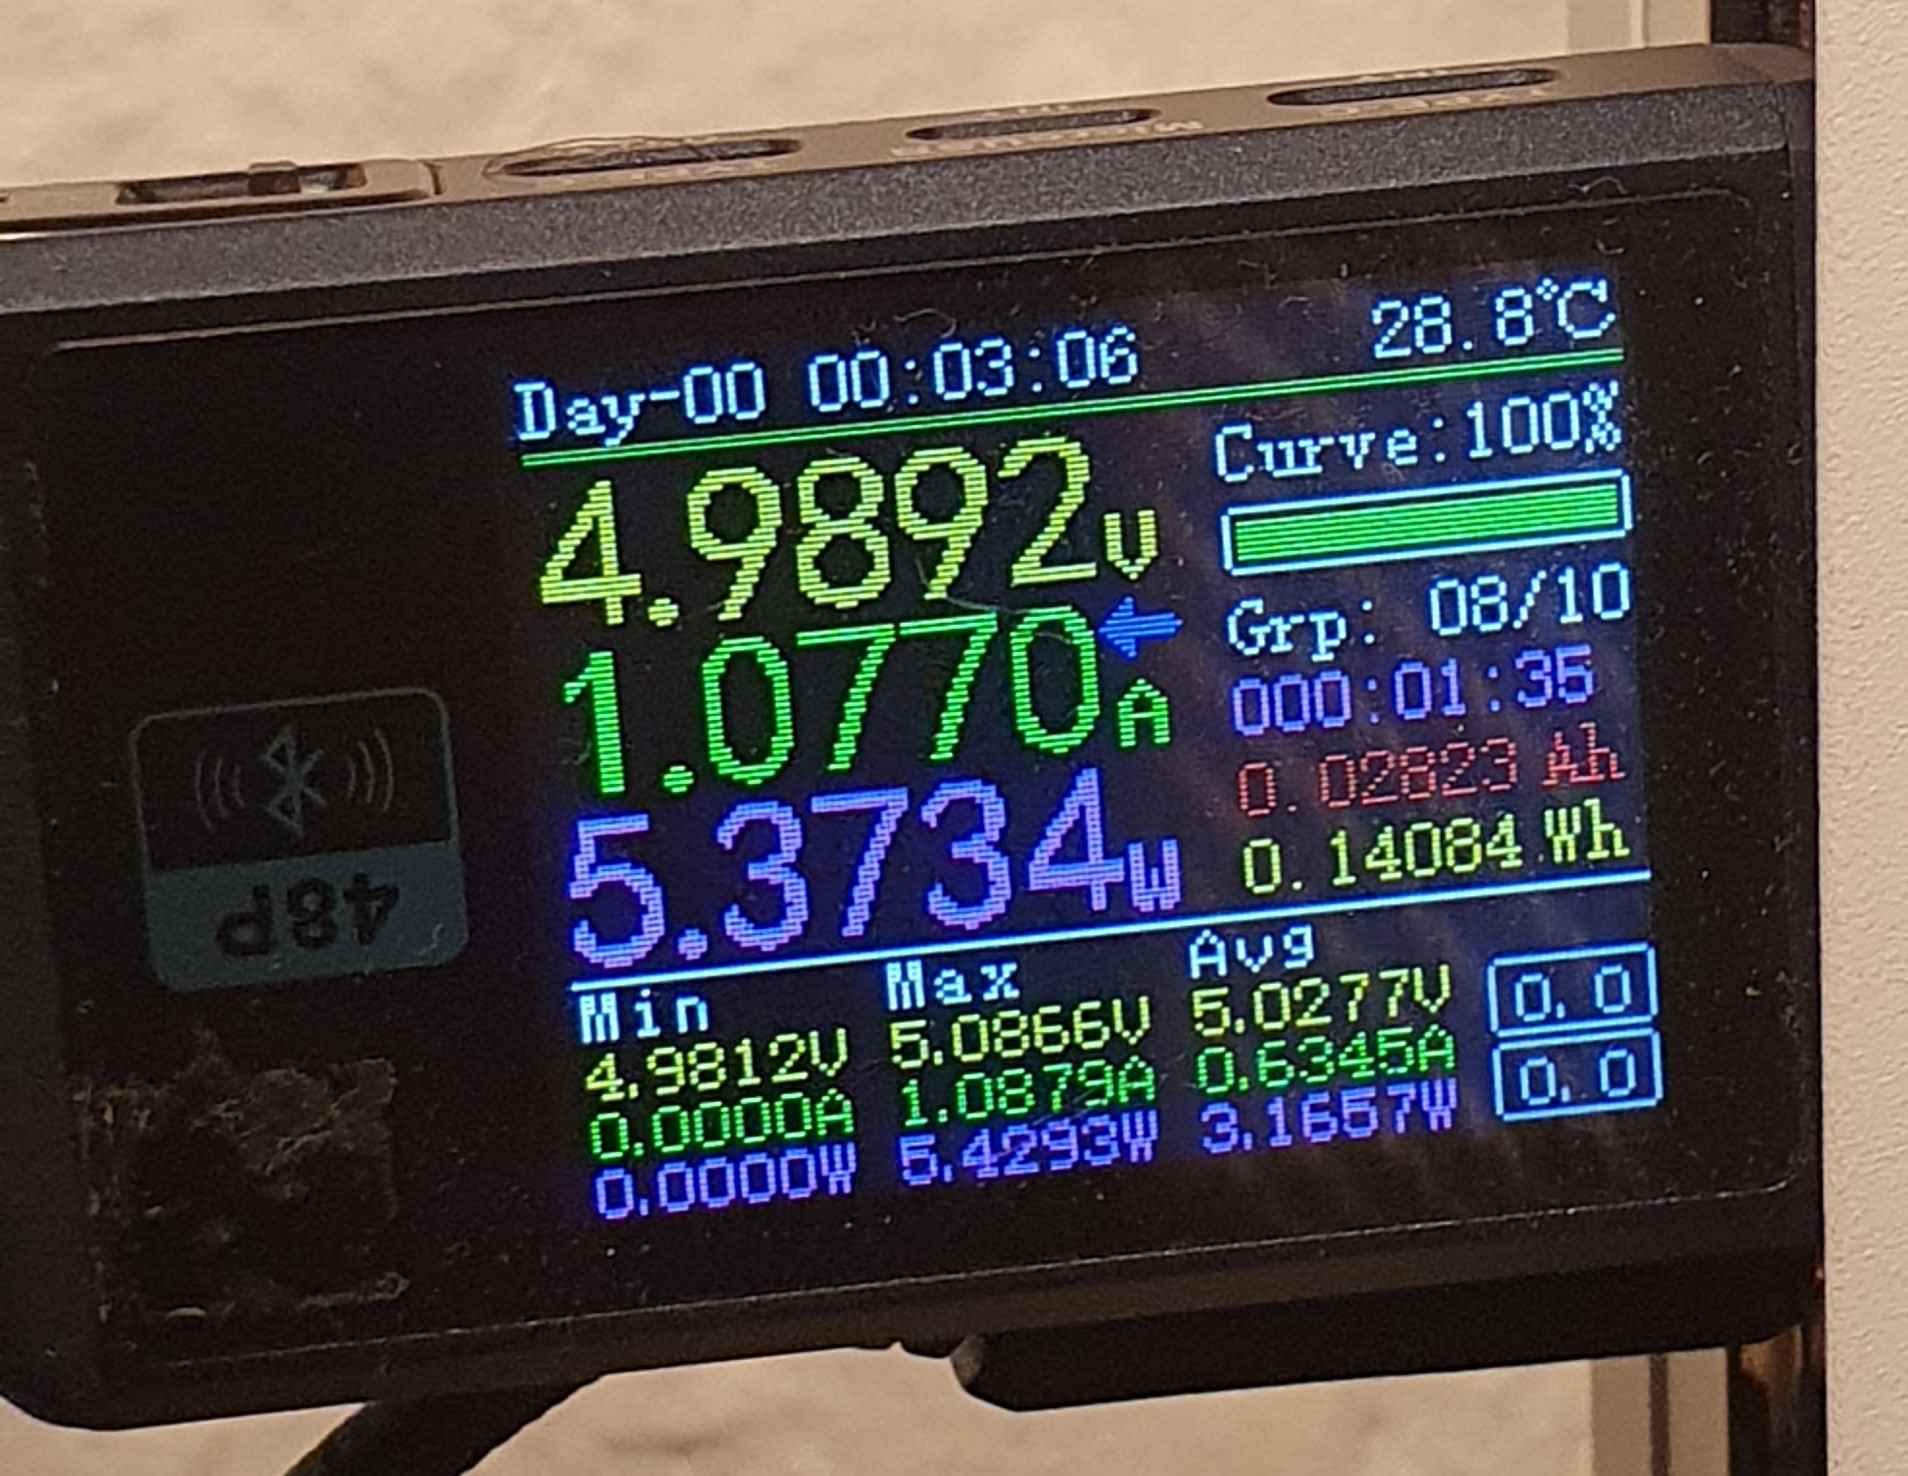
\includegraphics[width=0.5\linewidth]{img/power_test/tx.jpg}
    \caption{Leistungsaufnahme im Sendezustand}
    \label{fig:pwr_tx}
\end{figure}

Sensoren Strom?
MCU Strom?

Gesamtsystem Mess / Ruhezustand <200mA bei 5V 1W
Transmitt zustand \~ 1A bei 5V 5W

Messzeit: Sensorabhängig, 1 min à 1W
Transmitt Zeit: 30s à 5W
Energie Mess+Transmitt vorgang = 210J 





Operationslänge des Systems

Vielleicht nen Plot und Simulation?



\subsubsection{Datenübertragung}
\subsubsection{Computer}
\subsubsection{Sensorik}
ADC
\subsubsection{PCB}
\subsubsection{Aktuatoren}
\begin{itemize}
    \item Stromversorgung
    \begin{itemize}
        \item Solarzelle
    \end{itemize}
    \begin{itemize}
        \item Batterie - LiPo
        \item LiPo Charge Controller
        \item MPPT Controller
    \end{itemize}
    \item Datenübertragung
    \begin{itemize}
        \item GSM
        \item optional LoRa
        \item ggf. Datenspeicherung SD - Karte
    \end{itemize}
    \item Computer
    \begin{itemize}
        \item ESP32
    \end{itemize}
    \item Sensorik ? - Gemacht von Anderen
    \begin{itemize}
        \item Wassertrübung TDS
        \item Sauerstoffsättigung
        \item Leitfähigkeit TRB
    \end{itemize}
    \item Low Power
    \begin{itemize}
        \item Adafruit Timer
    \end{itemize}
    \item ADC
    \begin{itemize}
        \item ESP32 Intern
        \item ggf. Externer ADC per I2C
    \end{itemize}
    \item ggf. Rückmeldung
    \begin{itemize}
        \item LEDS
        \item Bildschirm
    \end{itemize}
    \item PCB
    \begin{itemize}
        \item Modulare, austauschbare Bauweise
        \item 
    \end{itemize}
\end{itemize}

\subsection{Rahmenbedingungen}
Das entwickelte System soll primär in der Spreeboje zum Einsatz kommen.
Die Technik soll jedoch auf andere Sensoren und Konditionen erweiterbar sein.
(wie z.B. im Wald)
Allen Umgebungen liegt eine Urbanität und keine klare Versorgung mit Strom oder Internetzugang über \ac{WLAN} oder Ethernet zu Grunde.
Der Formfaktor soll auch limitiert sein, da \ac{PCB}s preislich mit Größe skalieren. 
Als Stromquelle wird der Zugang zu Sonnenenergie vorausgesetzt.




\section{Implementierung}

Erster Lochplatten Prototyp


Blockdiagramm von Aufbau

\subsection{Operationskonzept}

State Diagram was die Boje macht


\subsection{Experiment}

Hier im detail erklären was du gemacht hast. 
\subsection{Tests}

GSM Übertragung

Server HTTP post

\subsection{Energietests}

Solar, Strom Kalkulationen und Tests

\subsection{PCB - Design}
Kicad
Design Anforderung Passend in Tube-Gehäuse


Messen ob Blocking Dioden da sind, ansonsten einfügen


\subsection{Code}
\url{https://git.tu-berlin.de/alexandros444/bachelor-waldbojen}

Serverseitig:
- Python Webserver

Für die Programmierung des ESP32 wurde VS-Code mit der PlattformIO Umgebung genutzt.
Der Programmcode ist in C / C++ geschrieben.
Der Programmablauf ist in \ref{fig:state_diagram}  zu sehen.



